\documentclass{book}

%margenes del documento
\setlength{\textwidth}{155mm} %longitud horizontal del texto
\setlength{\oddsidemargin}{5mm} %margen del borde frontal
\setlength{\evensidemargin}{7mm}%margen del lomo

%paquetes usados
\usepackage[utf8]{inputenc}
\usepackage{multicol}
\usepackage{graphicx}
\graphicspath{{./FIguras/}}

\title{Control de conexi\'on a red de parques e\'olicos}
\date{}
\author{Emilio Lia\~no}

\renewcommand*\contentsname{\'Indice}
\renewcommand*\bibname{Referencias}
\renewcommand*\chaptername{Cap\'itulo}


\begin{document}
	\pagenumbering{gobble} %no numera
	%portada
\begin{figure}[h!]
\centering

\includegraphics[width=\textwidth]{Encabezado.PNG}
\end{figure}
\begin{center}
\LARGE
UNIVERSIDAD POLIT\'ECNICA DE MADRID \par
\vspace {10 mm}
ESCUELA T\'ECNICA SUPERIOR DE INGENIER\'IA Y DISEÑO INDUSTRIAL\par
\vspace {10 mm}
\LARGE
Grado en Ingenier\'ia electr\'onica industrial y autom\'atica \par
\vspace {10 mm}
\Huge
TRABAJO FIN DE GRADO \par
\vspace{20 mm}
\LARGE
\textbf{Control de conexi\'on a red de parques e\'olicos}\par
\vspace {10 mm}
Autor: Emilio Liaño de la Fuente \par
\vspace {10 mm}
\end{center}
\newpage
   \par
\newpage
\normalsize
\pagenumbering{arabic}
\tableofcontents
\chapter{Introducci\'on}
	\section{Objetivos}
\chapter{Parques e\'olicos y conexi\'on a red}
Un parque e\'olico es una agrupaci\'on de aerogeneradores que transforman la energ\'ia e\'olica en energ\'ia el\'ectrica. En este cap\'itulo se har\'a una introducci\'on a los elementos de un parque e\'olico prestando especial atenci\'on a los elementos el\'ectricos y de control. Primero se expondran los elementos en general de un p\'arque e\'olico y de la conexi\'on a la red, despues se hablara de los parametros el\'ectricos del circuito de conexi\'on y de su comportamiento, y por \'ultimo se hablara de los c\'odigos de red y de las limitaciones que estos inponen sobre el funcionamiento de los parques e\'olicos.  
	\section{Elementos del parque}
Los parques e\'olicos necesitan para su funcionamiento los aerogeneradores para transformar la energ\'ia e\'olica en energ\'ia el\'ectrica, un sistema de control central y una red interna para la conexi\'on el\'ectrica. A su vez estos est\'an compuestos por diferentes elementos.

		\paragraph{Aerogenerador}
		Los aerogeneradores funcionan convirtiendo la energ\'ia cin\'etica del viento en energ\'ia mec\'anica rotatoria y esta, en energ\'ia el\'ectrica en una m\'aquina trif\'asica. Hay dos tipos seg\'un la disposici\'on de sus aspas, los de eje horizontal y los de eje vertical. A nivel industrial la impuesta es el eje horizontal por su rendimiento, fiabilidad y la capacidad de adaptarse a diferentes potencias. Este tipo de aerogenerador consta de un rotor, una multiplicadora, un generador trif\'asico, la conexi\'on a la red y un sistema de control. \par
		El rotor tiene las aspas que normalmente son tres, se puede variar la orientaci\'on de las palas en funci\'on de la velocidad del viento o de la potencia deseada. La multiplicadora transforma la baja velocidad y alto par del eje del rotor en alta velocidad y un par bajo en el eje del generador el\'ectrico, no todos los modelos lo incluyen necesariamente pero su uso est\'a muy extendido. El generador trif\'asico puede ser s\'incrono  o as\'incrono, esto depende de la topolog\'ia de conexi\'on que se utilice.  \par
		La conexi\'on a red se puede hacer de forma directa, para lo que se utiliza un generador as\'incrono de jaula de ardilla. Este tipo de conexi\'on se conoce tambi\'en como conexi\'on de velocidad fija porque la velocidad del rotor depende directamente de la frecuencia de la red, que normalmente es fija. En este sistema, a pesar de robusto por su sencillez se necesitan resistencias rot\'oricas para aumentar el rango de velocidades del viento con las que se puede trabajar, adicionalmente hay que incluir un banco de condensadores para compensar la potencia reactiva, ocasionando posibles resonancias en la red \cite{TopologiasWT}. \par 
		Otro tipo de conexi\'on es la doblemente alimentada, para esta configuraci\'on tambi\'en se usan m\'aquinas as\'incronas. En esta topolog\'ia el estator se encuentra conectado de forma directa a  la red como encontr\'abamos antes, pero el rotor est\'a conectado tambi\'en a la red por medio de un circuito de electr\'onica de potencia, consistente de un convertidor AC-DC-AC ‘back to back’ \cite{AerogeneradorDIFG}. Este tipo de topolog\'ia aumenta el rango de velocidades para generar potencia activa, la velocidad m\'axima estar\'a limitada a la potencia del convertidor, adem\'as permite tener un control sobre el factor de potencia de la m\'aquina, requisito necesario para poder conectarse a la red el\'ectrica. \par
		Por \'ultimo, la tercera topolog\'ia de conexi\'on normalmente utilizada es la \emph{‘Full Converter’}. Con este tipo de conexi\'on a la red se suelen utilizar m\'aquinas s\'incronas. En esta conexi\'on el estator est\'a conectado a la red a trav\'es de un convertidor ‘back to back’, sin ninguna conexi\'on adicional. En cuanto al rango de velocidades y el control de reactiva ofrece caracter\'isticas parecidas al doblemente alimentado, pero existen diferencias en coste. El doblemente alimentado es m\'as barato que el \emph{‘Full Converter’} inicialmente pero necesita un mantenimiento m\'as caro y ofrece menos potencia de salida anual \cite{PMGvsDFIG}. Ambos dos requieren un controlador de los transistores IGBT para su funcionamiento que los hace m\'as sofisticados.  \par
		Adem\'as del control de la salida el\'ectrica hay un controlador en cada torre para asegurar la seguridad y eficiencia del aerogenerador a nivel mec\'anico y aerodin\'amico. Por medio de m\'odulos para el control de equipos de potencia, el controlador de la turbina recibe la informaci\'on de los par\'ametros monitorizados y manipula los interruptores, bombas hidr\'aulicas, v\'alvulas y motores para controlar dichos par\'ametros. Estos controladores a su vez se comunican con un controlador central de todo el parque \cite{ComunicationControl}.  \par

		\paragraph {Controlador}
		El sistema de control de la planta incluye el propio controlador, la comunicaci\'on interna del parque y el SCADA, \emph{Supervisory Control And Data Acquisition} en español Supervisi\'on, Control y Adquisici\'on de Datos, para operar el sistema. Debido al aumento de los parques e\'olicos con una gran potencia y su penetraci\'on en la red, es necesario que estos se comporten como componentes activos controlables de la red apoyando su estabilidad. Para eso es necesario instalar un sistema de control central del parque. Este control es responsable de que el parque funcione de forma segura, \'optima y cumpliendo los reglamentos impuestos por la red el\'ectrica a la que este alimentando. \par
		Uno de los principales requerimientos que se especifican en la normativa del parque est\'a referido a los huecos de tensi\'on en la red. El objetivo es evitar la p\'erdida significativa de producci\'on de los aerogeneradores a lo largo de la duraci\'on de la falta. Los requerimientos de control se refieren a diferentes aspectos de la potencia del sistema y la estabilidad. \par 
		Dependiendo del estado de la red, el operador del sistema realiza demandas espec\'ificas al control central del parque, el cual prepara las señales de consigna a cada aerogenerador en concreto. El controlador central se encarga de cumplir los requerimientos del operador de red mandando las referencias de potencia activa y reactiva que se necesita de cada aerogenerador. Estas consignas se calculan con las medidas obtenidas en el PCC, \emph{Point of common coupling} en español punto de acoplamiento com\'un, y con la potencia disponible que ofrece cada rotor \cite{WindFarmController}.  \par
		La red de comunicaci\'on del parque est\'a formada por los controladores de los aerogeneradores, que est\'an instalados en la torre de cada turbina, que se comunican con el controlador central.  A su vez los controladores de cada torre recogen toda la informaci\'on necesaria de los modulos, que est\'an conectados con los instrumentos de medida a trav\'es de  un sistema de sensores. As\'i la red est\'a estructurada de forma jer\'arquica an\'aloga a los diferntes niveles de control como se ve en la figura \ref {ComLvls}. Los controladores de los aerogeneradores mandan toda la informaci\'on al controlador central y asignan las consignas que manda este dentro del aerogenerador \cite{ComunicationControl}.  \par
		Adem\'as de los modulos instalados en cada turbina, la red de control cuenta con diferentes modulos de control conectados a al controlador central. Entre otros el modulo de la l\'inea, el del trasformador, los de los buses de comunicaci\'on y los conectados a las redes de alimentaci\'on de los aerogeneradores. Estos modulos monitorizan las condiciones de operaci\'on como los desequilibrios de tensi\'on, el sobrecalentamiento, fases inversas, sincronizaci\'on pobre y los l\'imites de tensi\'on y frecuencia\cite{ComunicationControl}.   \par
		La red t\'ipica de un sistema de comunicaciones consiste de una conexi\'on principal de amplio ancho de banda y redes de bajo ancho de banda conectadas individualmente a la principal. La fibra \'optica y las microondas de radio suelen ser las tecnolog\'ias usadas para la comunicaci\'on principal. En las redes secundarias se suele utilizar cable de par trenzado de cobre, aunque se pueden usar tambi\'en sistemas inal\'ambricos. Generalmente en el caso de los parques e\'olicos se suelen utilizar PLCs, \emph{Power Line Communications} en español comunicaci\'on por l\'inea de potencia. Las tecnolog\'ias de PLCs disponibles permiten una gran velocidad transmisi\'on llegando a los 200 Mb/s. La principal ventaja de este tipo de comunicaci\'on es que las señales viajan a trav\'es de los mismos cables de la l\'inea el\'ectrica. Por otro lado estos cables suelen estar desprotegidos contra interferencias electromagn\'eticas y los m\'odulos que utilizan son m\'as caros que los de la comunicaci\'on inal\'ambrica \cite{ComunicationWF}. \par
	
	\section{Elementos de la conexi\'on a red}
	
	La red del parque est\'a formada por l\'inea de media tensi\'on que conecta con todos los aerogeneradores, la l\'inea de alta tensi\'on que ser\'ia la red el\'ectrica general a la que se le aporta la potencia y una subestaci\'on que contiene varios elementos. El PCC est\'a a un lado del transformador, dependiendo de si las medidas se toman del lado de baja o de alta tensi\'on es el criterio utilizado para dictaminar donde est\'a el PCC. \par
		\paragraph {L\'ineas de transmisi\'on}
Las l\'ineas de media tensi\'on generalmente en los parques conectan todos los aerogeneradores con el transformador con diferentes topolog\'ias. Las formas de conectar las l\'ineas de alimentaci\'on de los aerogeneradores son numerosas pero generalmente se utiliza la radial, la radial bifurcada, la de alimentaci\'on-subalimentaci\'on y en bucle. \par

La conexi\'on radial consiste de un solo cable de alimentaci\'on que se conecta secuencialmente a todos los aerogeneradores del parque, es la m\'as simple y por tanto la m\'as barata, es la que mejor se adapta para parques con los aerogeneradores en l\'inea. La radial bifurcada es parecida a la radial pero la l\'inea se divide para poder alimentar a dos series de aerogeneradores en paralelo, es la m\'as barata pero un fallo en la l\'inea supone una p\'erdida de todos los aerogeneradores. La alimentaci\'on-subalimentaci\'on junta varios cables de alimentaci\'on en radial en uno principal manteniendo los elementos de seguridad de cada cable de alimentaci\'on secundario, generalmente se usan para parques de gran tamaño que est\'an distribuidos en una gran \'area. La topolog\'ia en bucle conecta todos los cables secundarios de alimentaci\'on secundarios para evitar que un fallo en una de las l\'ineas la deje inoperante, es la m\'as segura de todas las topolog\'ias \cite{ComunicationTopologies}.\par
		\paragraph {Subestaci\'on}
El cable de alimentaci\'on general llega a la subestaci\'on donde se transforma la media tensi\'on en alta con un transformador. Dentro de la subestaci\'on, adem\'as de los componentes de los lados de media y alta tensi\'on, podemos encontrar los sistemas de medida y control, sistemas de protecci\'on contra incendios u otras incidencias y un sistema para ajustar la potencia reactiva. Tradicionalmente este sistema consistia de un sistema mecanico de bajo coste que conectaba un banco de condensadores. A pesar de que estos dispositivos ayudan a mejorar el factor de potencia y la regulaci\'on de tensi\'on en estado estacionario, no se puede resolver satisfactoriamente problemas como las fluctuaciones de potencia o tensi\'on y la eliminaci\'on de harm\'onicos. \par

La integraci\'on de los aprque e\'olicos a la red requiere una compensaci\'on de la potencia reactiva din\'amica para apoyar a la estabilidad, sobre todo durante perturbaciones en la red. Para conseguir un alto rendimiento en el control de la tensi\'on tanto en transitorio como estacionario en el PCC se utilizan FACTS, \emph{flexible ac transmission system} en español sistema flexible de transmisi\'on en corriente continua. Los dos m\'as comunes usados en parques e\'olicos son el SVC, \emph{static var compensator}, y el STATCOM, \emph{static synchronous compensator} \cite{FACTS}.  \par

El STATCOM suele ser la opci\'on considerada para esta soluci\'on por las ventajas que presenta frente al SVC. Entre estas ventajas se encuentra un tiempo de respuesta m\'as r\'apido y una capacidad de aporte de tensi\'on auxilair mayor por su naturaleza de fuente de tensi\'on \cite{STATCOM}. \par

En el lado de media tensi\'on se suele encontrar el barraje que conecta la red al cuadro el\'electrico, el seccionador para abrir el circuito cuando no hay corriente y un interruptor autom\'atico para abrir el circuito ante corientes el\'ectricas elevadas. En el lado de alta tensi\'on suele haber reactancia a tierra en los transformadores, una toma a tierra general, descargadores de sobretensi\'on, otro seccionador y otro disyuntor.  \par


	\section{Par\'ametros de la red trif\'asica} 
	
	Todas las l\'ineas el\'ectricas descritas en la secci\'on anterior son trif\'asicas por las ventajas que este tipo de redes presentan frente a las monof\'asicas. En esta secci\'on se cubrir\'an todos los par\'ametros que hay que controlar de una red trif\'asica, su sentido f\'isico y las operaciones que los relacionan. \par

El circuito que se va a analizar se puede reducir a una fuente de intensidad que ser\'ia al conjunto de aerogeneradores, una l\'inea que une esta fuente con el primario del transformador y otra l\'inea que une el secundario con la red, que estar\'ia representada por una fuente de tensi\'on. En los parques e\'olicos reales las medidas de los par\'ametros de la red solo se realizan a un lado del transformador, pero para analizar el circuito en esta secci\'on colocare medidores a ambos lados. Los par\'ametros de la red que se observan y controlan en un parque e\'olico son la tensi\'on, la intensidad, la potencia, tanto activa, reactiva y aparente y la frecuencia. \par

Para la medici\'on de estos valores se considera que los circuitos de la red de conexi\'on son equilibrados, por lo que las tensiones de cada fase y las intensidades tendr\'an el mismo valor eficaz y un desfase de 120º entre s\'i. Para expresar esta diferencia de fase se suele utilizar la notaci\'on fasorial,  pero por la simplicidad a la hora de hacer ciertos c\'alculos como la suma o la resta se usan n\'umeros complejos para definir los vectores tambi\'en. Para poner una referencia a la fase se le da a un valor de tensi\'on o corriente el valor 0 o 90 de fase. En este caso, para tomar el mismo crit\'erio que los resultados de Simulink, se dar\'a fase 0 a la intensidad de la primera fase, $I_a$. \par

Las fuentes de intensidad generan tres ondas sinusoidales de igual amplitud y desfasadas entre ellas 120º. Conectada a una carga se pueden observar tambien tres ondas sinusoidales de voltage que tambi\'en son equilibradas. Entre las ondas de tensi\'on e intensidad existe una relaci\'on dada por la impedancia de la carga representada en la ley de Ohm. \par
\begin{equation}\label{eq:ohm}
	\overline{I}=\overline{V}/\overline{Z}
\end{equation} \par
Si los par\'ametros de la ecuaci\'on son introducidos como fasores y teniendo en cuenta que la fase de la intensidad se considera 0, podemos concluir que el desfase entre la intensidad y la tensi\'on viene dado por la fase de la carga y la relaci\'on entre los m\'odulos es el m\'odulo de la impedancia. Si la impedancia es puramente resistiva el desfase es nulo entre ambas, si es de car\'acter capacitivo la intensidad va adelantada y si es de car\'acter inductivo la intensidad va retrasada respecto a la tensi\'on. \par

Para observar este efecto de la carga sobre la relaci\'on entre tensi\'on e intensidad se simula el circuito de la figura \ref{LoadAnalyserModel} y cambiando los valores de la impedancia se obtienen las gr\'aficas de la figura \ref {Va_IaALL}, en las que se puede ver en el transitorio como la intensidad de la primera fase, $I_a$,  se adelanta o se retrasa respecto a la tensi\'on, $V_a$, dependiendo del tipo de carga.  \par

\begin{figure}[h!]
\centering
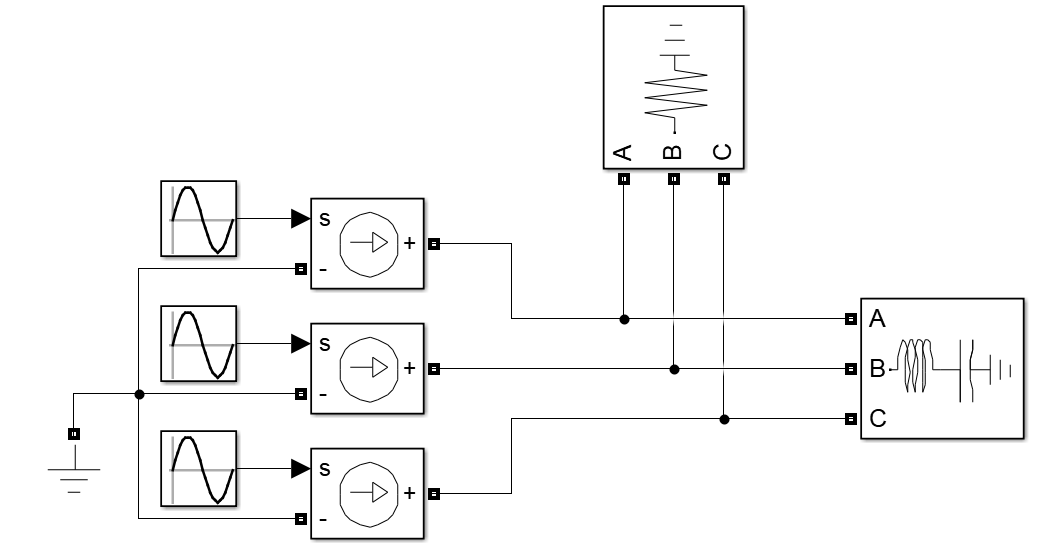
\includegraphics[width=0.9\textwidth]{LoadAnalyserModel.PNG}
\caption{Modelo de una carga alimentada por una fuente de intensidad trif\'asica en Simulink}
\label{LoadAnalyserModel}
\end{figure}

\begin{figure}[h!]
\centering
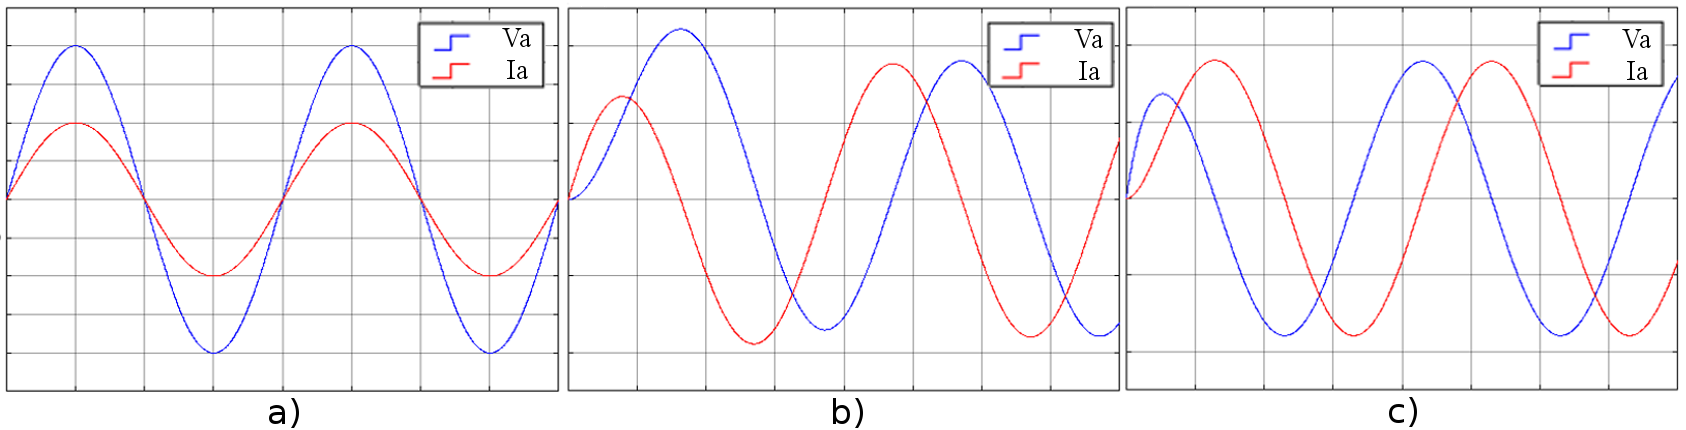
\includegraphics[width=1\textwidth]{Va_IaALL.PNG}
\caption{Respuesta del circuito ante carga resistiva a), capacitiva b) e inductiva c).}
\label{Va_IaALL}
\end{figure}

Cuando la carga es puramente capacitiva o inductiva se produce un desfase entre la intensidad y la tensi\'on de 90º. Si la carga es capacitiva, al estar la intensidad adelantada respecto a la tensi\'on el angulo visto desde la tensi\'on sera positivo y si la carga es inductiva el angulo sera negativo visto desde la tensi\'on como se puede ver en la figura \ref {PhasComp}. Para todos los calculos de potencias el angulo se ve desde la tensi\'on a la intesidad, por eso se utiliza ese criterio de signos. \par

\begin{figure}[h!]
\centering
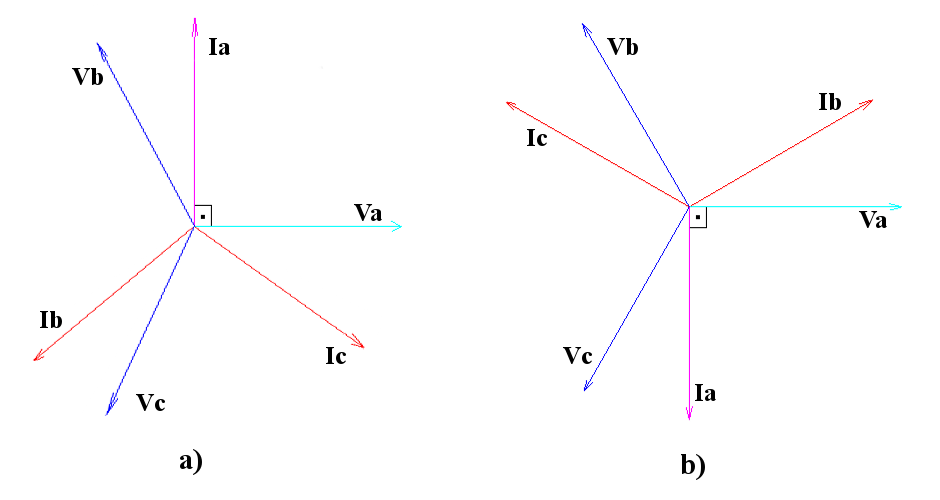
\includegraphics[width=1\textwidth]{PhasComp.PNG}
\caption{Fasores de una carga puramente capacitiva a) e inductiva b).}
\label{PhasComp}
\end{figure}

En el an\'alisis de la conexi\'on a red es importante la potencia, esta debe cumplir con los requisitos que marcan el operario de red y el c\'odigo de red. Para el c\'alculo de la potencia de una red trif\'asica se utiliza la siguiente f\'ormula:   \par

\begin{equation}
	\overline{S}=\sqrt{3} \overline{V}_L  \overline{I}_L^*
\end{equation} \par

Podemos observar que la potencia consumida o sumisnistrada por un elemento del circuito tiene una componenente real y una componenente imaginaria que se llaman potencia activa, $P$ y reactiva, $Q$ respectivamente. Desarrollando la formula anterior usando complejos llegamos a lo siguiente: \par

\begin{equation}\label{eq:potensia}
	\overline{S}= \sqrt{3} V_L I_L \cos{\varphi}+j\sqrt{3} V_L I_L \sin{\varphi} = P+jQ 
\end{equation} \par

Donde $\varphi= \alpha_V-\alpha_I$. Por lo tanto basandose en el criterio de signos anteriormente mencionado para los \'angulos trataremos la $Q$ negativa como capacitiva y con signo positiva como inductiva. \par

\'Analizando la diferencia de tensi\'on entre dos puntos de un circuito que esta descrita por la ecuaci\'on (\ref{eq:ohm}), donde la tensi\'on antes de la carga es $E$ y la tensi\'on despues de la carga es $V$ tenemos que:

\begin{equation}\label{eq:difV}
	\Delta V=E-V=ZI
\end{equation} \par

 Introduciendo la ecuaci\'on (\ref{eq:potensia}) en la ecuaci\'on (\ref{eq:difV}) obtenemos el siguiente desarrollo:
\begin{equation}\label{eq:lol}
	\Delta V=(R+jX)\frac{P-jQ}{E}= \frac{RP+XQ}{E}+j\frac{XP-RQ}{E}
\end{equation} \par

Cuando hablamos de una linea de transmisi\'on, como son las que conectan el parque con al subestaci\'on y esta con la red, consideramos que $X \gg R$ \cite{WFgridcode}. Considerando entonces despreciable el valor de $R$ en la formula (\ref{eq:lol}) queda lo siguiente: 
\begin{equation}
	\Delta V= Q\frac{X}{E}+jP\frac{X}{E}
\end{equation} \par

Esto significa que los cambios en la magnitud de de la tensi\'on son controlados por la potencia reactiva y la  diferencia de fase entre emisor y receptor viene dada por la potencia activa \cite{WFgridcode}. Por eso se utiliza el control de la potencia activa y reactiva para controlar frecuencia de la red y la tensi\'on respectivamente. \par

Normalmente la fercuencia es m\'as estable que la tensi\'on en la red el\'ectrica por lo que los p\'arques e\'olicos tratan de producir la potencia el\'ectrica m\'axima que permita la instalaci\'on y la demanda de la red, y as\'i obtener los mayores beneficios posibles. Es por eso la reactiva la que suele variar m\'as para mejorar la claidad de la potencia entregada. 


	\section{C\'odigos de red}

Un c\'odigo de red es un conjunto de especificaciones t\'ecnicas que definen los par\'ametros que debe cumplir una instalci\'on para asegurar la seguridad y estabilidad de la red p\'ublica a la que est\'a conectada  \cite{UKgridCode}. Dichas instalaciones pueden ser plantas el\'ectricas generadoras, consumidores u otra red. En este apartado se prestara especial atenci\'on a los c\'odigos de red referidos a plantas el\'ectricas y al c\'odigo de red de España en concreto. \par

Los c\'odigos de red var\'ian seg\'un la red para la que se han diseñado. Es por eso cada pa\'is tiene un c\'odigo de red propio, pero no solo var\'ia de un pa\'is a otro si no que incluso dentro de España las condiciones que se imponen en la red peninsular o no peninsulares son distintas por las diferencias en las redes y las condiciones en las que operan. A pesar de las diferentes restricciones, los casos que se abordan en los codigos de red suelen ser comunes para la mayor\'ia de ellos.  \par

En el caso de la conexi\'on y operaci\'on de plantas generadoras los requerimientos m\'as importantes para el control son los rangos de frecuencia y tensi\'on, el control de la potencia activa y el control de la reactiva en operaci\'on normal. Tambien se cubren los casos de perturbaciones en la red como los huecos de tensi\'on o la inyecci\'on de corriente reactiva. Normalmente estos requerimientos pueden ser descritos como las siguientes zonas de operaci\'on para frecuencia y voltaje. Operaci\'on continua en un rango limitado alrededor del punto nominal, operaci\'on por tiempo limitado con una posible reducci\'on de la salida en unos margenes extendidos y por \'ultimo la desconexi\'on inmediata \cite{GridCodeDeepAnalisys}.\par

		\paragraph{Tensi\'on}
Respecto al control de tensi\'on, en la secci\'on anterior se ha visto que la magnitud de la tensi\'on esta controlada por la potencia reactiva. Por lo tanto el control de la tensi\'on se expone en los c\'odigos de red como un control de la potencia reactiva en funci\'on de la tensi\'on de red \cite{WFgridcode}. En los PO, procedimientos de operaci\'on que forman el c\'odigo de red de España, el control de la potencia reactiva esta definido por la potencia activa neta instalada del parque. En el PO 7.4 \cite{PO74}  se establece que todos los generadores deben funcionar dentro de el margen de generaci\'on/absorci\'on que aparecen en la figura \ref{VQgridcode}.   \par 

\begin{figure}[h!]
\centering
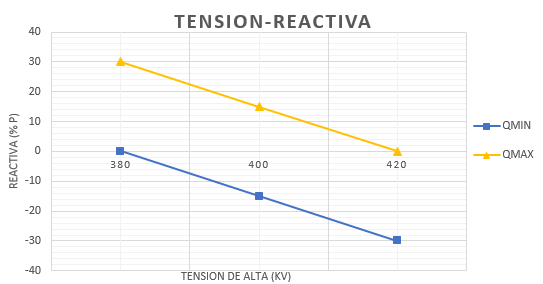
\includegraphics[width=0.8\textwidth]{VQgridcode.PNG}
\caption{L\'imites de potencia reactiva en funci\'on de la tensi\'on de la linea}
\label{VQgridcode}
\end{figure}
\newpage
		\paragraph{Frecuencia}
Como consecuencia de un desajuste entre la potencia activa aportada y la demanda se produce un cambio en la energía almacenada en la masa rotativa del generador que provoca un desvio de la frecuencia del sistema. Un aumento en la potencia entregada se convertir\'ia en un aumento de la velocidad angular del generador y por tanto un aumento de frecuencia, pasando lo contrario al entregar potencia por debajo de la demanda \cite{WFgridcode}, \cite{FrecuencyLvL}. \par

Normalmente el control de la frecuencia esta compuesto por tres funciones distintas. El control primario de frecuencia, usado ante los desequilibrios repentinos en la red. Actua a nivel local en la turbina en un rango de 15 a 30 segundos. El control secundario o de carga permite reestablecer la frecuencia y la potencia a los valores programados. Se realiza en las unidades de control central del p\'arque y actua en un rango de 15 minutos. Este es el tipo de funci\'on que se implementara en este trabajo. Finalmente esta el control terciario que consiste en la gesti\'on de la potencia generada por cada aerogenerador para ayudar al control secundario \cite{WFgridcode}. \par





\chapter{Control de plantas el\'ectricas}

La teor\'ia de control es un campo de la ingenier\'ia y las matem\'aticas que trata el comportamiento de los sistemas din\'amicos. El problema de control consiste en, dada una entrada o referencia a un actuador en un sistema f\'isico o planta, obtener la respuesta deseada de dicha planta. \par

Esto se puede conseguir en lazo abiertoo  en lazo cerrado. La solución en lazo abierto es, conociendo las condiciones de la planta y su funci\'on de transferencia, introducir una referencia con la que se obtenga la salida deseada. En lazo cerrado se realimenta comparandola con la entrada para medir el error del sistema, este error generalmente entra a un controlador que da finalmente la entrada a la planta con la que se obtiene la salida deseada. Este esquema de realimentaci\'on se muestra en la figura \ref{FeedBackLoop} y es en los que se basan normalmente los controladores usados en la industria. \par

\begin{figure}[h!]
\centering
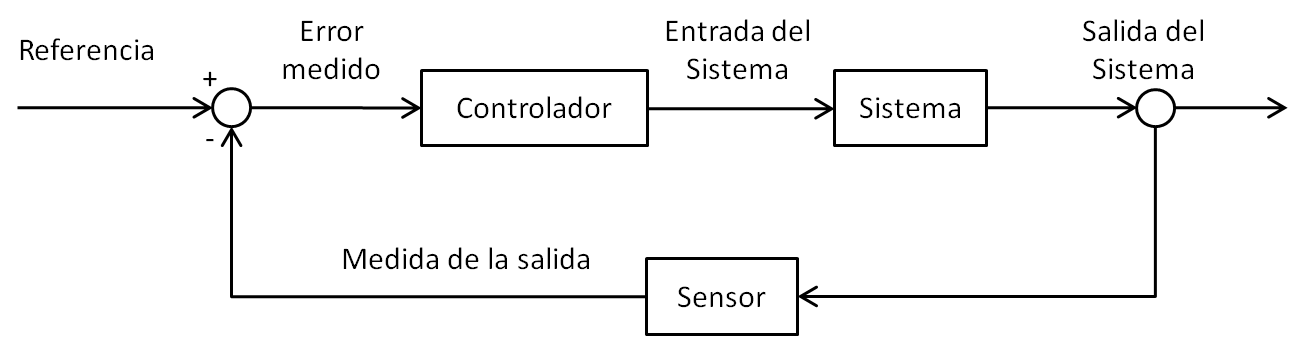
\includegraphics[width=1\textwidth]{Realimentacion.PNG}
\caption{Esquema de control en lazo cerrado.}
\label{FeedBackLoop}
\end{figure}

Por la complejidad del sistema de conexi\'on a red de una planta electrica y la posibilidad de variaciones en sus parametros a lo largo del tiempo en este cap\'itulo se hablara de la soluci\'on de lazo cerrado. Primero se hablara del control en general de plantas el\'ectricas y se definira el concepto de los niveles de control, en la siguietne secci\'on se establecer\'a el estado del arte en el control de parques e\'olicos y a contiunaci\'on se hablara de las t\'ecnicas de control cl\'asicas y modernas existentes. \par 

	\section{Introducci\'on al control de plantas el\'ectricas}

	\section{Estrategias de control utilizadas}

	\section{Control cl\'asico}

	\section{Control mod\'erno}

\chapter{Herramientas de diseño}


	\section{Desarrollo en Simulink de un modelo matem\'atico del parque}

Para el desarrollo del modelo su simulaci\'on se utilizar\'a la herramienta de programaci\'on Simulink. Simulink es un entorno de programaci\'on de diagramas de bloques para el diseño basado en modelos. Es parte del entorno de programaci\'on de Matlab pero a un nivel de abstracci\'on m\'as alto que el lenguaje interpretado usado en los scripts. \par

Simulink permite diseñar y simular modelos de sistemas f\'isicos y sistemas de control por medio de diagramas de bloques. El comportamiento de dichos sistemas se define mediante operaciones matem\'aticas, señales predefinidas y funciones de Matlab. Adem\'as de las multiples herramientas de desarrollo Simulink cuenta con una serie de utilidades para la visualizaci\'on, \'analisis y guardado de los resultados de cada simulaci\'on. Con estas caracter\'isticas Simulink es una herramienta ampliamente usada en modelado de sistemas el\'ectricos y electr\'onicos, tanto como para ingenier\'ia de control. \par

El modelo de Simulink se compondra de tres partes. El modelo electrico de la red, que se montara usado la liber\'ia Simscape Power Systems de Simulink como se explicara m\'as adelante. El lazo de ralimentaci\'on y control que se compondria de todas las herramientas matematicas para manejar los datos leidos de la red y controlarla. Por \'ultimo, esta la parte de visualizaci\'on y an\'alisis de los datos con la que se estudiara el modelo y el control que se diseñen.   \par

		\paragraph{Control} 
Con el control se trata de que el modelo alcance unos valores de potencia activa y reactiva establecidos como consignas, $P^*$ y $Q^*$. Con estas dos consignas se calcula la consigna de potencia aparente, $S^*$, como n\'umero complejo que servira de consigna \'unica. Para eso se realimentaran las medidas de tensi\'on e intensidad de las tres fases, $V_{abc}$ e $I_{abc}$. \par

Con las medidas tomadas de $V_{abc}$ e $I_{abc}$ en el lado de alta tensi\'on se calcula la potencia activa y reactiva del circuito en ese punto. Las medidas de tensi\'on e intensidad se pueden tomar tanto en el lado de alta como de media tensi\'on del transformador, la situaci\'on del medidor depende del parque en concreto. En este caso eleg\'i medir en el lado de alta porque estas medidas son las que realmente estan afectando a la estabilidad de la red. \par

Las medidas de potencia activa y reactiva en el lado de alta tensi\'on se utilizan para calcular la potencia aparente en forma de complejo. Esta potencia aparente se resta a la consigna cerrando el lazo de realimentaci\'on. Esta diferencia es el error en potencia aparente del sistema que entra en el bloque de control, en el caso del control cl\'asico un PID. A la salida del control se opera la señal de potencia aparente para que vuelva a dar una intensidad que se introduce a las fuentes de intensidad del modelo el\'ectrico.  \par

		\paragraph{Observaci\'on}
Para poder analizar el comportamiento del modelo el\'ectrico Simulink tiene herramientas de observación y seguimiento de las variables. Dentro de la libreria b\'asica de Simulink podemos encontrar en el apartado de \emph{Sinks} algunas de estas herramientas. Existe tanto la opci\'on de guardar los valores de la simulaci\'on como la visualizaci\'on de las gr\'aficas. \par

Usando el bloque \emph{To Workspace} podemos guardar la evoluci\'on de una variable a lo largo de una simulaci\'on como vector o como estructura con tiempo.  \par

		\subsection{Librer\'ia Simscape Power Systems}

La liber\'ia Simscape Power Systems contiene elementos y herramientas de \'analisis para el modelado y simulaci\'on de sistemas el\'ectricos. Entre otros incluye elementos de redes trif\'asicas y sistemas de energ\'ias renovables. Todo el modelo del circuito el\'ectrico esta realizado con elementos de esta librer\'ia. La propia librer\'ia tiene tambien las herramientas para simular y calcular el modelo ofreciendo diferentes opciones al usuario seg\'un que tipo de resultados necesite. \par

		\paragraph {Simulaci\'on}
El bl\'oque \emph{Powergui} permite elegir entre tres m\'etodos de resolver el modelo del circuito. Estos son continua, discreto y fasorial. Adem\'as este bloque te permite establecer ciertos par\'ametros globales para la simulaci\'on como el tiempo de muestreo o la frecuencia.  \par

La simulaci\'on por el metodo de continua resuelve el modelo con el tiempo discreto m\'as pequeño que le permitan los recursos del ordenador. Al no tener un tiempo de muestreo fijo los resultados pueden cambiar de una simulaci\'on a otra. Con este m\'etodo de resoluci\'on se puede observar el valor instantaneo de las medidas. Adem\'as tambien calcula  los transitorios de elementos como bobinas o condensadores que tienen una inercia. \par

El modo discreto fija un tiempo de muestre que el usuario elige. Las propiedades son las mismas que en el modo continuo pero los resultados son siempre los mismos independientemente de lo que se tarde en hacer los c\'alculos. Ambos m\'etodos se utilizan para simulaciones de periodos de tiempo cortos en las que es necesario analizar la forma de onda o en aquellos modelos que sea necesario estudiar sus etapas trasnitorias. \par

El m\'etodo fasorial calcula todos los valores de tensi\'on e intensidad como vectores, ya sean fasores o complejos. 

		\paragraph {Fuentes el\'ectricas}

		\paragraph {Medidores}

		\paragraph {L\'ineas de transmisi\'on}
Las l\'ineas de transmisi\'on son elementos pasivos del circuito que presentan una impedancia. Para definir una l\'inea de media distancia, que son las que se utilizan en un parque e\'olico, hay dos t\'ipos de par\'ametros. Existen los par\'ametros transversales, la conductancia y la capacidad, y est\'an los  par\'ametros longitudinales, resistencia e inductancia. Existen dos formas de agrupar estos par\'ametros, el circuito equivalente en $T$ y el circuito equivalente en $\pi$ \cite{LibroRedesLineas}. En este trabajo voy a centrarme en el modelo $\pi$ que es el que usare en el modelo de Simulink.  \par

El circuito equivalente en $\pi$ mantiene unidos los par\'ametros longitudinales y divide los par\'ametros transversales. En el tramo central se sit\'uan la resistencia y la reactancia mientras que la conductancia y capacitancia quedan divididas en los extremos con sus valores a la mitad, $G/2$ y $B/2$. El circuito est\'a representado en la figura \ref{CircuitoPi}. \par 

\begin{figure}[h!]
\centering
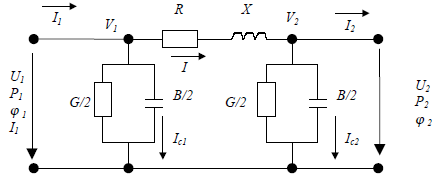
\includegraphics[width=0.7\textwidth]{CircuitoPi.PNG}
\caption{Circuito equivalente de circuito $\pi$ \cite{LibroRedesLineas}. }
\label{CircuitoPi}
\end{figure} \par

En el modelo de Simulink para definir la l\'inea con el circuito equivalente  $\pi$ se deben introducir los valores con los que simulink calcula las resistencias, inductancias y capacitancias formando el circuito equivalente que se muestra en la figura \ref{PiSectionSimulink}.  \par 

\begin{figure}[h!]
\centering
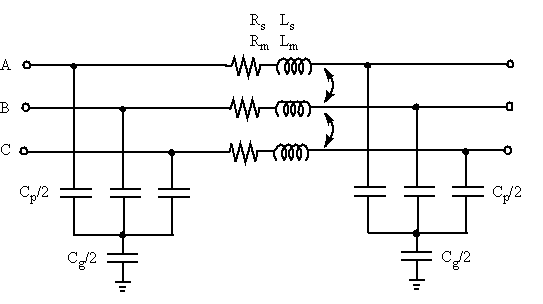
\includegraphics[width=0.6\textwidth]{PiSectionSimulink.PNG}
\caption{Circuito equivalente de circuito $\pi$ utilizado por Simulink. }
\label{PiSectionSimulink}
\end{figure} \par

		\paragraph{Transformador}

		\subsection{Tratamiento de señal por buses}

Simulink trabaja usando señales para comunicar los bloques. El tratamiento de estas señales es importante por ser precisamente estas a las que se las hara el seguimiento en las simulaciones. Para el tratamiento de multiples señales existe la herramienta de los buses. Los buses son estructuras formadas por varias señales o incluso otros buses. \par

Los buses se manejan dentro del modelo con 

		\subsection{Diseño encapsulado mediante modelos referenciados}

\chapter{Modelado y simulaci\'on del control}

	\section{Desarrollo de un modelo de parque y red de conexi\'on}

	\section{Modelado del parque y la conexi\'on a red en Simulink}

	\section{Diseño del control de la conexi\'on a red}

	\section{Casos de estudio}

\chapter{An\'alisis de resultados}


\chapter{Conclusiones y estudios futuros}

\bibliography{Biblio}
\bibliographystyle{ieeetr}
\end{document}